The natural generalization of MPS to higher dimensional lattices is given by \textit{Projected Entangled Pair States} (PEPS). A PEPS is constructed similar to a MPS by representing the local subsystem on each lattice site $i$ with the index $\sigma_i$ of a tensor $T_i^{\sigma_i}$ and connecting nearest-neighbour tensors with virtual bonds. The quantum state can then be written as
\begin{equation}
	\label{eq:PEPS_definition_general}
	\left|\Psi\right\rangle = \sum_{\sigma_1,\sigma_2,\dots,\sigma_N} \mathcal{C}\left(T_1^{\sigma_1}, T_2^{\sigma_2}, \dots, T_N^{\sigma_N}\right) \left|\sigma_1,\sigma_2,\dots,\sigma_N\right\rangle,
\end{equation}
where $\mathcal{C}(\dots)$ denotes the contraction of the full network along all virtual bonds. As an example, we draw a PEPS on a square lattice in figure \figref{fig:square_PEPS}. \par
\begin{figure}
	\centering
	\subcaptionbox{\label{fig:square_PEPS}}
	{%
		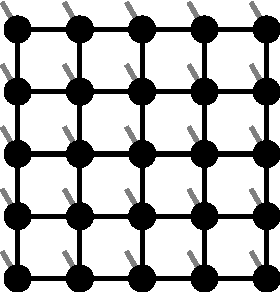
\includegraphics[scale=1]{figures/tikz/Tensor_Networks/isoTPS_structure/isoTPS_structure_a.pdf}
	}
	\quad\quad
	\subcaptionbox{\label{fig:square_isoTPS}}
	{%
		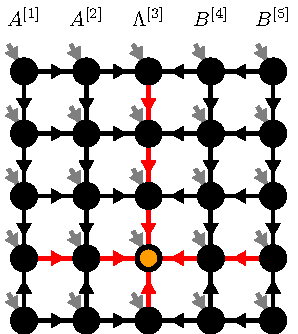
\includegraphics[scale=1]{figures/tikz/Tensor_Networks/isoTPS_structure/isoTPS_structure_b.pdf}
	}
	\caption{Tensor Networks representing two dimensional states on a square lattice. (a) A Projected Entangled Pair State (PEPS). (b) An isometric Tensor Product State (isoTPS). \todo{Include orthogonality center tensor}}
	\label{fig:square_PEPS_and_isoTPS}
\end{figure}
PEPS are able to efficiently represent area-law states in two and higher dimensions \cite{cite:practical_introduction_MPS_and_PEPS}. Remarkably, PEPS can even handle correlations decaying polynomially with separation distance \cite{cite:criticality_the_area_law_and_the_computational_power_of_PEPS}, whereas MPS can only handle exponentially decaying correlations. Polynomially decaying correlations are characteristic for critical points. \par
Unfortunately, it is not generally possible to bring a PEPS into an exact canonical form due to the presence of closed loops. Thus, already the computation of local expectation values scales exponentially with system size and can in practice be only done approximately, e.g. using the boundary MPS method \cite{cite:practical_introduction_MPS_and_PEPS} or corner transfer matrices \cite{cite:CTMRG}. Moreover, algorithms for ground state search and time evolution have computational costs scaling with high powers of the bond dimension. For example the cost of a full update TEBD or DMRG iteration is dominated by the contraction of an effective environment, scaling as $\mathcal{O}\left(D^{10}\right)$ \cite{cite:unifying_PEPS_contractions}. \par
Recently, the new class of \textit{isometric Tensor Product States} (isoTPS) has been introduced \cite{cite:isometric_tensor_network_states_in_two_dimensions, cite:conversion_of_PEPS_into_a_canonical_form, cite:DMRG_approach_to_optimizing_2D_tensor_networks}, generalizing the canonical form of MPS to higher dimensions by enforcing isometry constraints. This allows for efficient computation of local expectation values and greatly lowers the cost of some algorithms. The downside to this approach is that the set of states representable by isoTPS is smaller than the set of state representable by PEPS. It is thus an interesting question to ask which kinds of states and, more generally, which kinds of quantum phases can still be represented by isoTPS. \par
In the following, we will give a brief introduction to the isoTPS defined in \cite{cite:isometric_tensor_network_states_in_two_dimensions} and discuss their properties. A two-dimensional isoTPS on the square lattice is constructed by enforcing the isometry conditions shown in figure \figref{fig:square_isoTPS}. All isometries are chosen in such a way that all arrows point towards a special row and column, called the \textit{orthogonality hypersurface} of the isoTPS. The term "hypersurface" is chosen in anticipation of a generalization to higher dimensions. Because of the isometry condition, one can think of the contractions of each of the four regions outside the orthogonality hypersurface as orthogonal boundary maps \cite{cite:efficient_simulation_of_dynamics_in_two_dimensional_quantum_spin_systems}. The single tensor with only incoming arrows is called the \textit{orthogonality center}. local expectation values of operators acting in the vicinity of the orthogonality center can be computed efficiently because most contractions reduce to identity, similar to the computation of local expectation values in MPS (see figure \figref{fig:mps_local_expectation_value_canonical}). The orthogonality center can be moved along the orthogonality hypersurface simply and exactly using a QR-decomposition as shown in figure \figref{fig:isoTPS_moving_ortho_center}. \par
\begin{figure}
	\centering
	\subcaptionbox{\label{fig:isoTPS_moving_ortho_center}}
	{%
		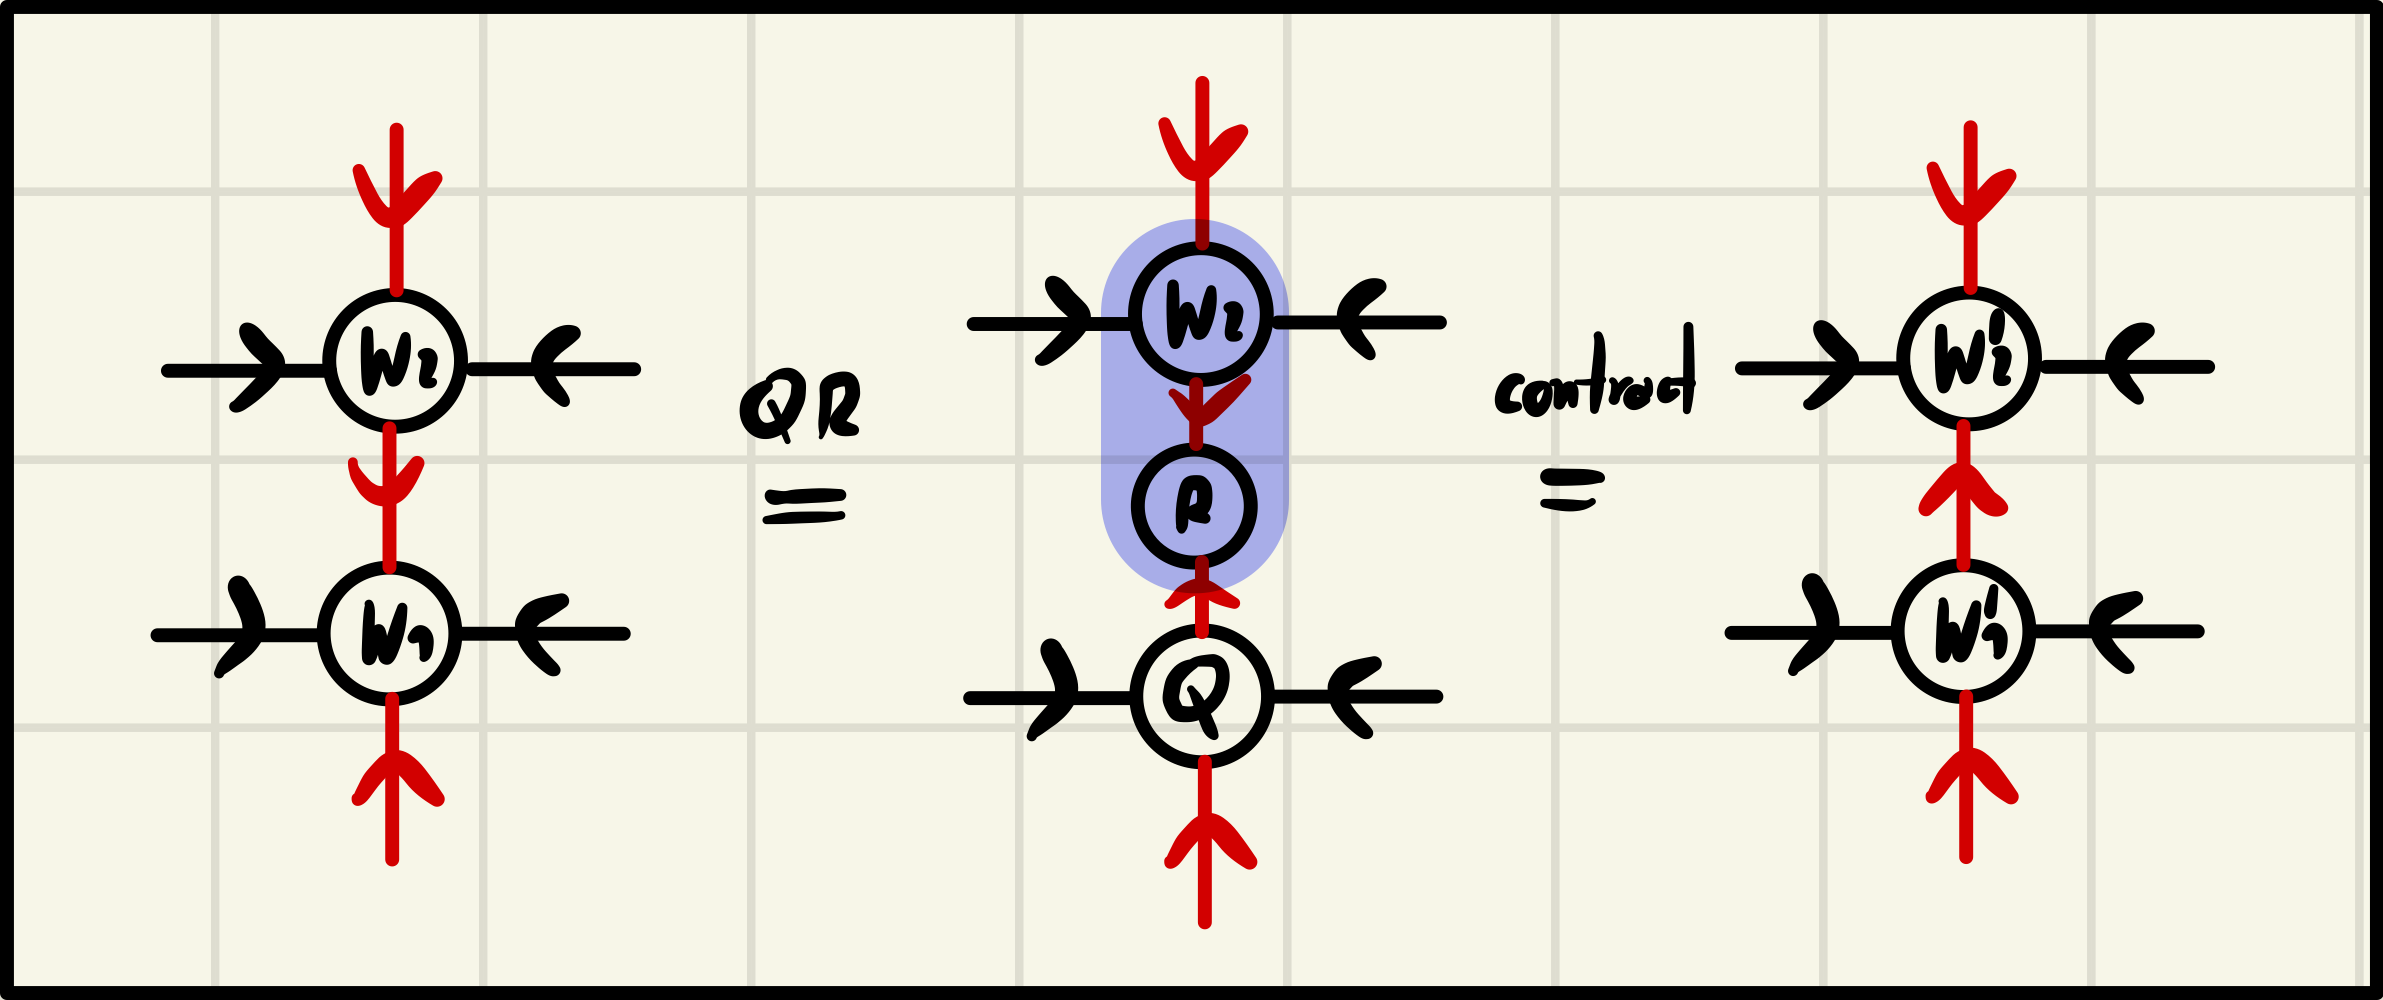
\includegraphics[width=0.3\textwidth]{figures/Tensor_Networks/Moving_ortho_center.jpeg}
	}
	\subcaptionbox{\label{fig:isoTPS_moving_ortho_column}}
	{%
		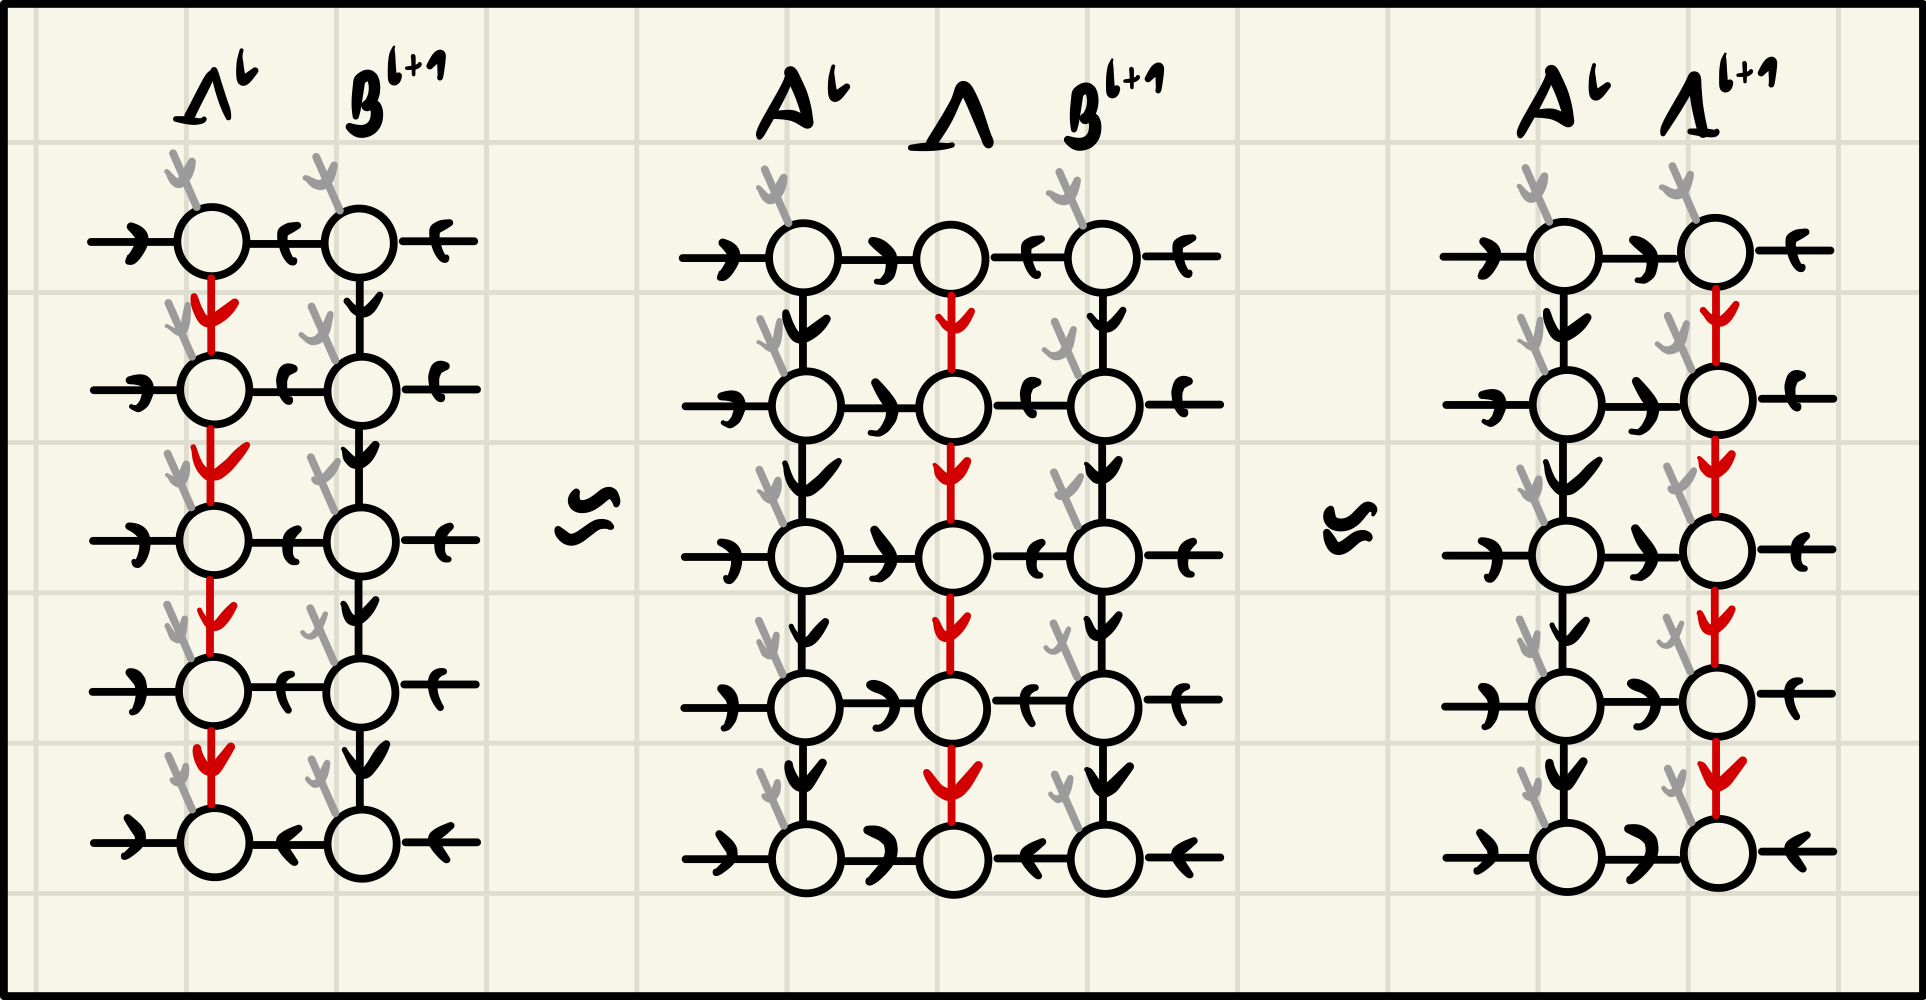
\includegraphics[width=0.6\textwidth]{figures/Tensor_Networks/variational_MM.jpeg}
	}
	\caption{Moving the orthogonality center and the orthogonality hyper surface around is a central problem in isoTPS applications. (a) Moving the orthogonality center along the orthogonality hypersurface can be done easily via QR-decompositions. (b) An orthogonality column can be moved by first solving equation \eqref{eq:isoTPS_moving_ortho_surface_auxillary_formulation} variationally and then absorbing $\Lambda$ into $B_{l+1}$ via the standard MPO-MPS multiplication and MPS compression algorithms.}
	\label{fig:isoTPS_moving_ortho_center_and_column}
\end{figure}
Moving the orthogonality surface is a harder problem, which in general can only be done approximately. In analogy to MPS and as shown in figure \figref{fig:square_isoTPS}, we call columns left of the orthogonality hypersurface $A_l$ and tensors right of the orthogonality hypersurface $B_l$, with $l = 1,2,\dots,L$ and $L$ the linear system size. Moving the orthogonality hypersurface $\Lambda_l$ one column to the right can be expressed as solving the problem
\begin{equation}
	\label{eq:isoTPS_moving_ortho_surface_general}
	\Lambda_l B_{l+1} = A_l \Lambda_{l+1},
\end{equation}
where the notation $\Lambda_l B_{l+1}$ means the contraction of columns $\Lambda_l$ and $B_{l+1}$ along their connecting bonds. Instead of \eqref{eq:isoTPS_moving_ortho_surface_general}, one can solve the simpler auxillary problem
\begin{equation}
	\label{eq:isoTPS_moving_ortho_surface_auxillary_formulation}
	\Lambda_l = A^l \Lambda,
\end{equation}
where $\Lambda$ is a column of tensors with no physical indices, as shown in figure \figref{fig:isoTPS_moving_ortho_column}. This column can then be absorbed into $B_{l+1}$ via the standard algorithm of applying an MPO to an MPS and subsequent MPS compression \cite{cite:DMRG_in_the_age_of_MPS}. One can variationally solve problem \eqref{eq:isoTPS_moving_ortho_surface_auxillary_formulation} by minimizing the distance $\left\lvert\Lambda_l-A_l\Lambda\right\rvert$, sweeping back and forth through the tensors while respecting the isometry condition.\todo{Maybe reference Evenbly-Vidal here?}
\begin{figure}
	\centering
	\subcaptionbox{\label{fig:Moses_move}}
	{%
		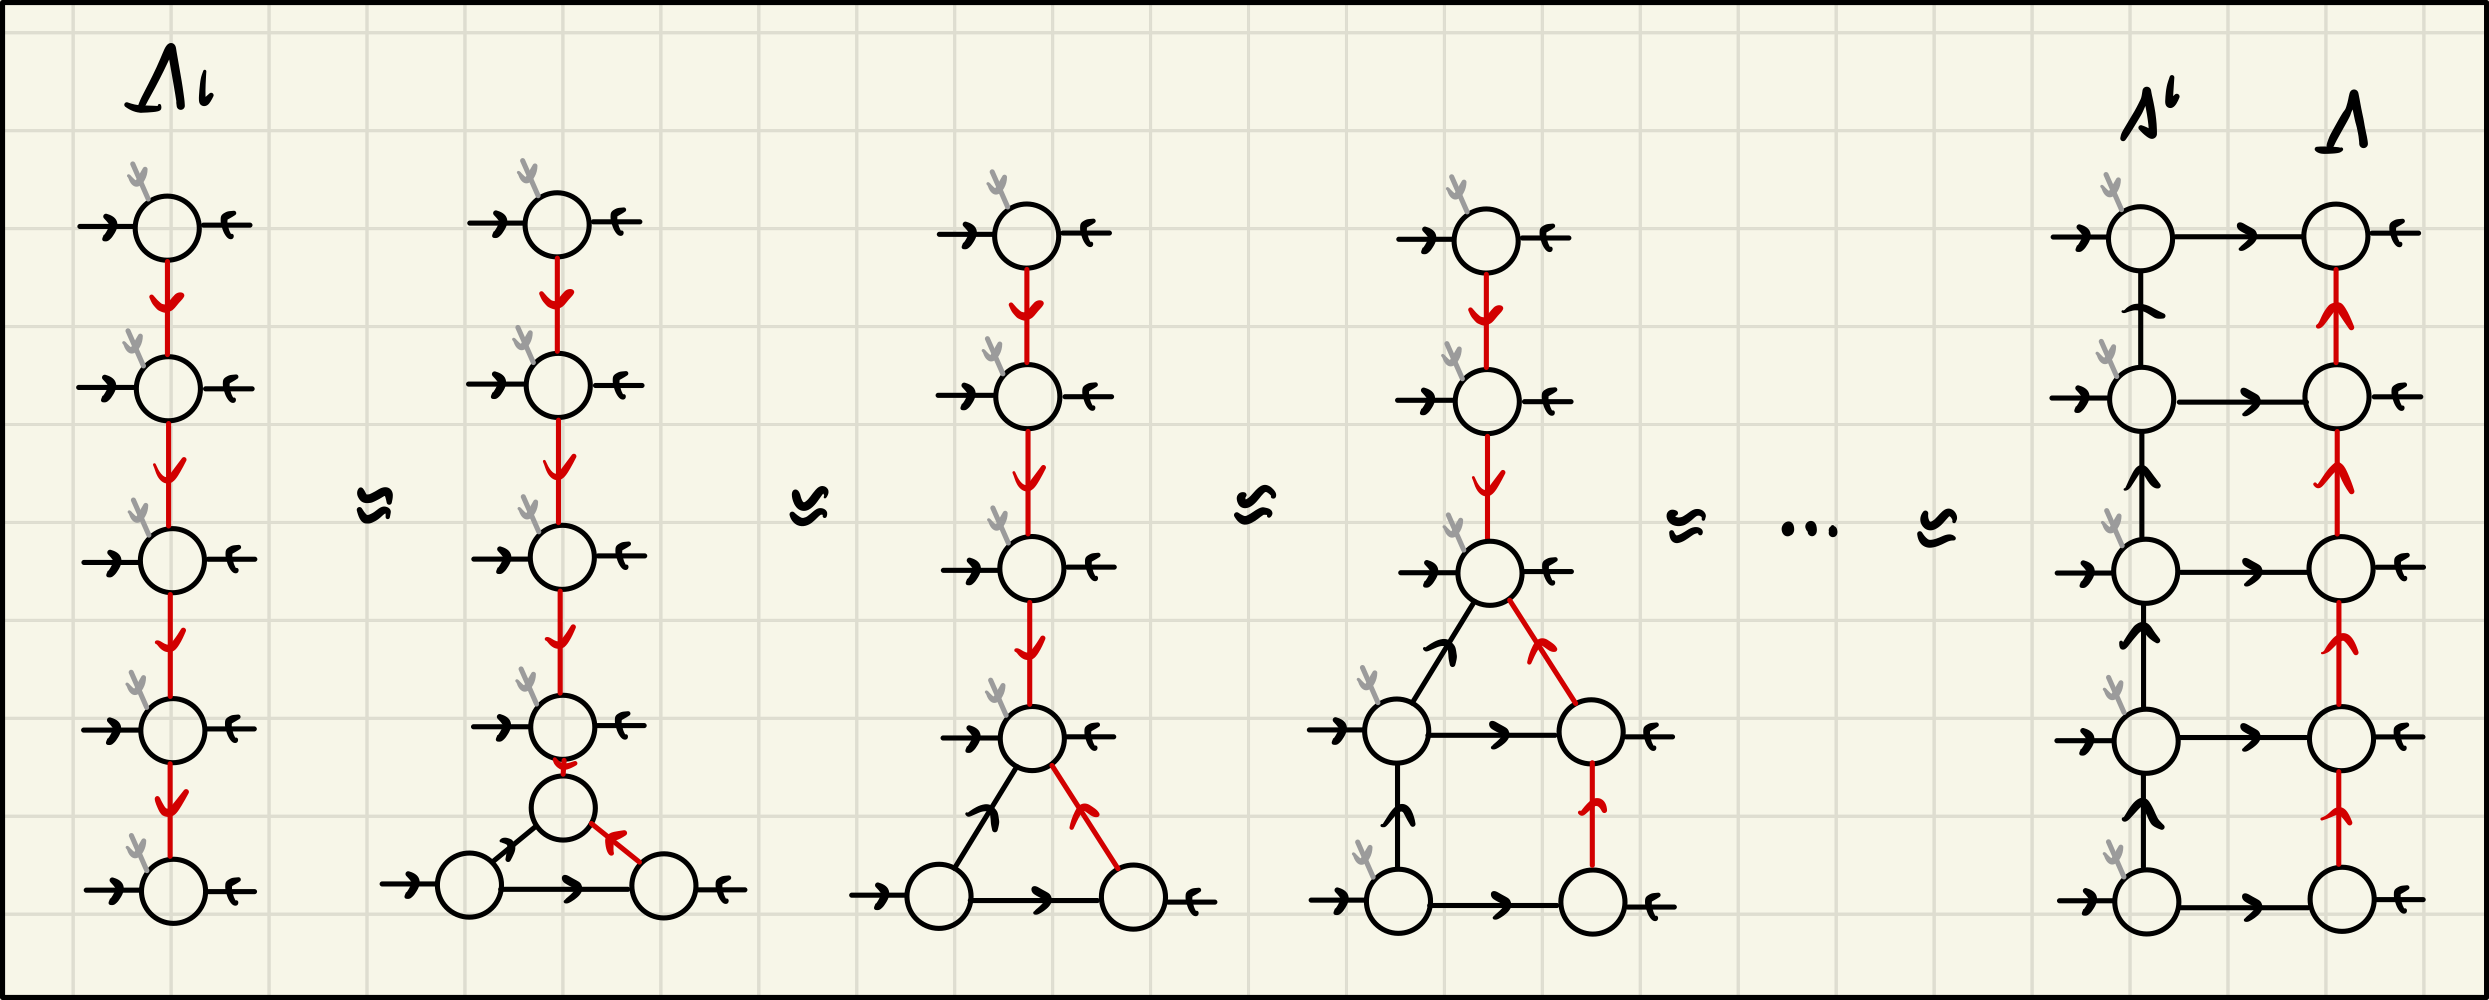
\includegraphics[width=0.8\textwidth]{figures/Tensor_Networks/MM.jpeg}
	}
	\subcaptionbox{\label{fig:tripartite_decomposition}}
	{%
		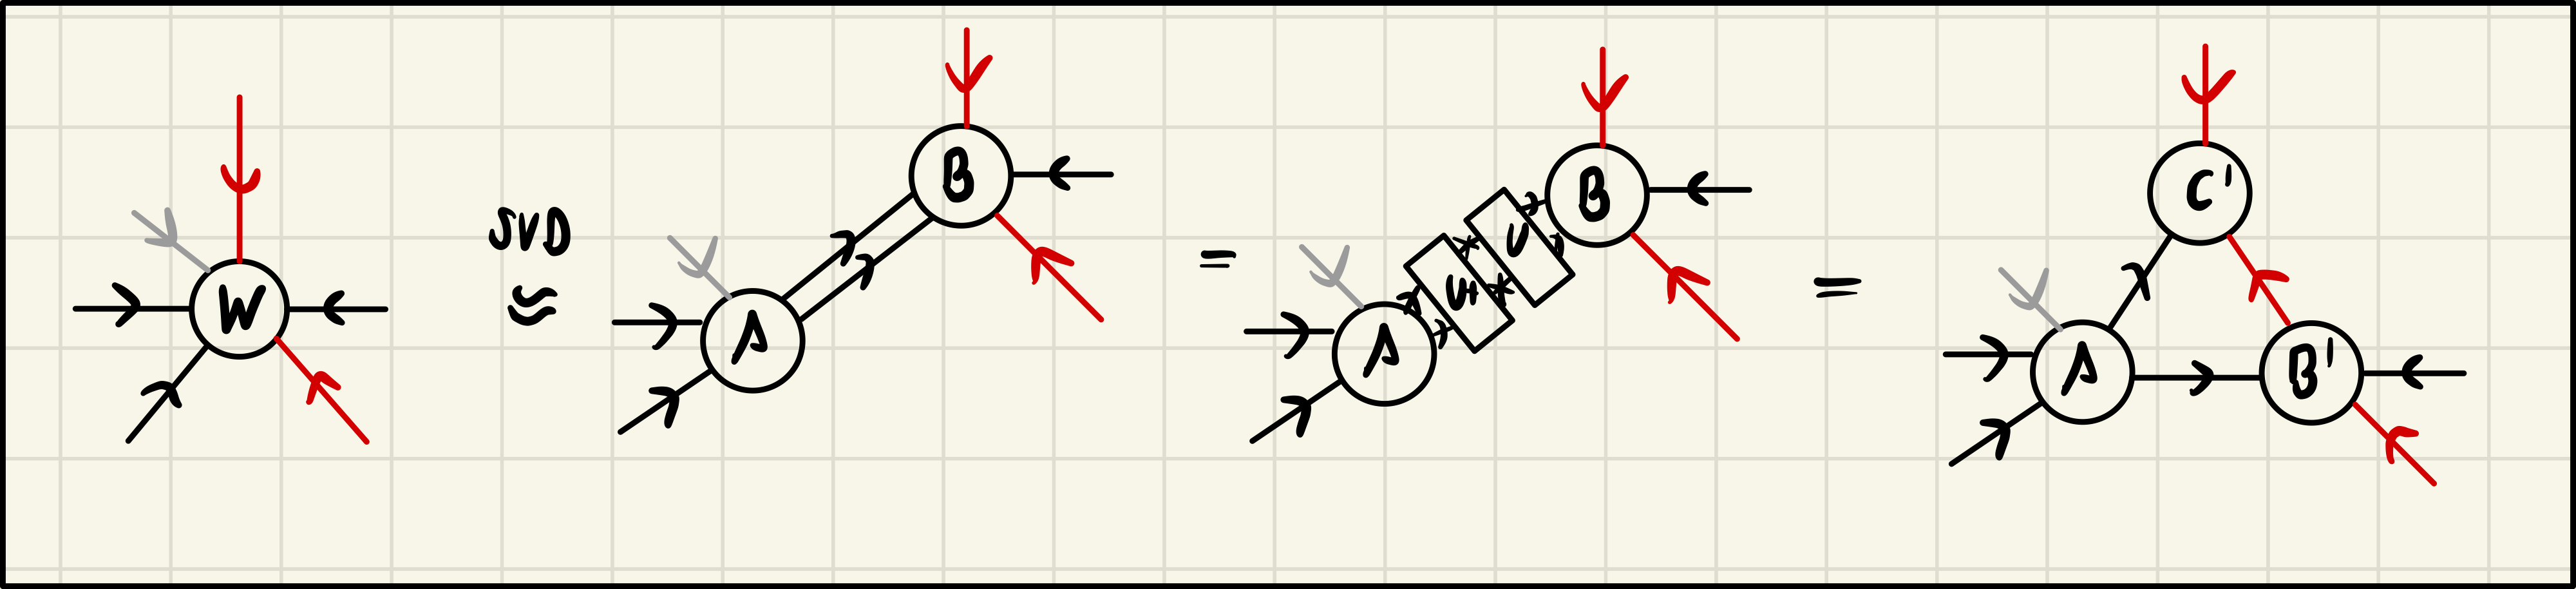
\includegraphics[width=0.8\textwidth]{figures/Tensor_Networks/Tripartite_decomposition.jpeg}
	}
	\caption{(a) The Moses Move (MM) splits the column $\Lambda_l$ into $A_l$ and $\Lambda$ via a single unzipping sweep of tripartite decompositions. (b) Tripartite decomposition of the tensor $W$ as explained in the text.}
	\label{fig:Moses_move_and_tripartite_decomposition}
\end{figure}
It is however found in \cite{cite:isometric_tensor_network_states_in_two_dimensions} that a single unzipping sweep, called the \textit{Moses Move} (MM), provides a solution very close to the variational one whilst being far quicker. The MM can also be used as a good initialization for the variational algorithm. We sketch the MM in figure \figref{fig:Moses_move}. We start from the bottom of the orthogonality hypersurface column and split the tensors one after the other using a tripartite decomposition. A single tripartite decomposition of a tensor $W$ is shown in figure \figref{fig:tripartite_decomposition}. First, $W$ is split into two tensors $A$ and $B$ via a truncated SVD $W = U(SV) = AB$ with $A$ an isometry. The bond connecting A and B is reshaped into two bonds. Next, it is important to note that the full contraction is invariant under the insertion of a unitary and its conjugate transpose, $AB = (AU^\dagger)(UB)$, with $(AU^\dagger)$ still satisfying the isometry condition. This degree of freedom can be used to \textit{disentangle} the tensor $B$ along the direction of the red bonds. Accordingly, we choose $U$ such that the truncation error or some entanglement measure is minimized for splits along the direction of the red bonds. Choosing a good disentangling unitary is crucial for a successful tripartite decomposition and will be discussed further in section \ref{sec:}. Assume for now that a good disentangling unitary has been found. After contracting $(AU^\dagger)$ and $(UB)$, a truncated SVD is used to split $(UB)$ into tensors $B^\prime$ and $C^\prime$ as shown in figure \figref{fig:tripartite_decomposition}, completing the tripartite decomposition. \par
Because the orthogonality center can be moved easily along the orthogonality hypersurface, one can think of the orthogonality hypersurface along a column or row as a 1D MPS with an enlarged physical bond dimension grouping together the phsical and the two ancilla legs pertruding from the orthogonality hypersurface tensors. Standard MPS algorithms can then be generalized to isoTPS by performing one iteration of the algorithm on the orthogonality hypersurface MPS, before moving the hypersurface via MM or variational optimization and repeating the procedure. As an example, we will discuss TEBD$^2$, the generalization of $TEBD$ to an isoTPS on a 2D square lattice. \todo{write}. \par
isoTPS are a new class of states that enable the implementation of faster algorithms for e.g. ground state search and time evolution, compared to PEPS. The expressional power of isoTPS has been studied in \cite{cite:isometric_tensor_network_representation_of_string_net_liquids}, where it was found that isoTPS with finite bond dimension can exactly represent ground state wavefunctions of string-net liquid models, showing that long-range entanglement does not form an obstruction for isoTPS representations and suggesting that the ground states of gapped Hamiltonians with gappable edges can be efficiently represented as an isoTPS. There have also been works discussing the computational complexity of isoTNS \cite{cite:computational_complexity_of_isometric_tensor_network_states} and relating isoTNS to quantum circuits \cite{cite:sequential_generation_of_projected_entangled_pair_states, cite:quantum_circuits_for_2D_isometric_tensor_networks}. In \cite{cite:topological_quantum_phase_transitions_in_2D_isometric_tensor_networks}, topological phase transitions were studied with isoTPS, showing that isoTPS can represent some critical states with power-law correlations. A DMRG$^2$-algorithm was implemented on isoTPS in \cite{cite:efficient_simulation_of_dynamics_in_two_dimensional_quantum_spin_systems} and used to compute dynamical structure factors of ground states using real time evolution. IsoTPS were also extended to fermionic systems \cite{cite:fermionic_isometric_tensor_network_states}, to two dimensional strips of infinite length \cite{cite:two_dimensional_isometric_tensor_networks_on_infinite_strip}, and to three dimensional cubic lattices \cite{cite:three_dimensional_isometric_tensor_networks}. They have also been used to compute properties of two dimensional thermal states \cite{cite:isometric_tensor_network_representation_of_2D_thermal_states}.